\documentclass[t]{beamer}
\usepackage{default}
\usepackage[]{graphicx}
\usepackage{amsfonts}
\usepackage{amssymb}
\usepackage{amsmath}
\usepackage[brazil]{babel}
\usepackage[utf8]{inputenc}
\usepackage[T1]{fontenc}
\usepackage{lmodern}
\usepackage{hyperref}
\usepackage{subcaption}
\usepackage{listings}
\usepackage[absolute,overlay]{textpos}
\usetheme{Dresden}
\setbeamertemplate{caption}[numbered]

\author{Thiago de Gouveia Nunes \\ Orientador: Prof. Marcel P. Jackowski}
\title{Aceleração de Registro Não-Rígido de Imagens em GPU}
\institute{IME - USP}

\setbeamertemplate{navigation symbols}{}
\setbeamertemplate{bibliography item}{}
\setbeamercolor{framesource}{fg=gray}
\setbeamerfont{framesource}{size=\tiny}

\newcommand{\frameofframes}{/}
\newcommand{\setframeofframes}[1]{\renewcommand{\frameofframes}{#1}}
\newcommand{\source}[2]{\begin{textblock*}{10cm}(#2cm,8.6cm)
    \begin{beamercolorbox}[ht=0.5cm,right]{framesource}
        \usebeamerfont{framesource}\usebeamercolor[fg]{framesource} Source: {#1}
    \end{beamercolorbox}
\end{textblock*}}

\setframeofframes{/}
\makeatletter
\setbeamertemplate{footline}
  {%
    \begin{beamercolorbox}[colsep=1.5pt]{upper separation line foot}
    \end{beamercolorbox}
    \begin{beamercolorbox}[ht=2.5ex,dp=1.125ex,%
      leftskip=.3cm,rightskip=.3cm plus1fil]{title in head/foot}%
      {\usebeamerfont{title in head/foot}\insertshorttitle}%
      \hfill%
      {\usebeamerfont{frame number}\usebeamercolor[fg]{frame number}\insertframenumber~\frameofframes~\inserttotalframenumber}
    \end{beamercolorbox}%
    \begin{beamercolorbox}[colsep=1.5pt]{lower separation line foot}
    \end{beamercolorbox}
  }
\makeatother

\lstset{ %
language=C,                  % choose the language of the code
basicstyle=\footnotesize,       % the size of the fonts that are used for the code
numbers=left,                   % where to put the line-numbers
numberstyle=\footnotesize,      % the size of the fonts that are used for the line-numbers
stepnumber=1,                   % the step between two line-numbers. If it's 1 each line will be numbered
numbersep=5pt,                  % how far the line-numbers are from the code
showspaces=false,               % show spaces adding particular underscores
showstringspaces=false,         % underline spaces within strings
showtabs=false,                 % show tabs within strings adding particular underscores
frame=single,                   % adds a frame around the code
framerule=0.6pt,
tabsize=2,                      % sets default tabsize to 2 spaces
captionpos=b,                   % sets the caption-position to bottom
breaklines=true,                % sets automatic line breaking
breakatwhitespace=false,        % sets if automatic breaks should only happen at whitespace
escapeinside={\%*}{*)},         % if you want to add a comment within your code
backgroundcolor=\color[rgb]{1.0,1.0,1.0}, % choose the background color.
rulecolor=\color[rgb]{0.8,0.8,0.8},
extendedchars=true,
xleftmargin=10pt,
xrightmargin=10pt,
framexleftmargin=10pt,
framexrightmargin=10pt
}

\begin{document}
\frame{\titlepage}

\section{Introdução}
\subsection{Introdução}

\begin{frame}
  O registro é o processo de alinhamento espacial ou geométrico entre duas ou mais imagens. 
Ele é uma etapa fundamental em uma série de aplicações:
  \begin{itemize}
    \item A criação de imagens panorâmicas
    \item A fusão de informações (imagens de diferentes modalidades)
    \item Correção de movimentação em imagens médicas
  \end{itemize}
\end{frame}

\begin{frame}
  \begin{figure}
    \begin{center}
      \includegraphics[width=0.55\textwidth]{figuras/costura.png}
      \source{http://en.wikipedia.org/wiki/Image\_registration}{2}
    \end{center}
  \end{figure}
\end{frame}

\begin{frame}
  \begin{figure}
    \begin{center}
      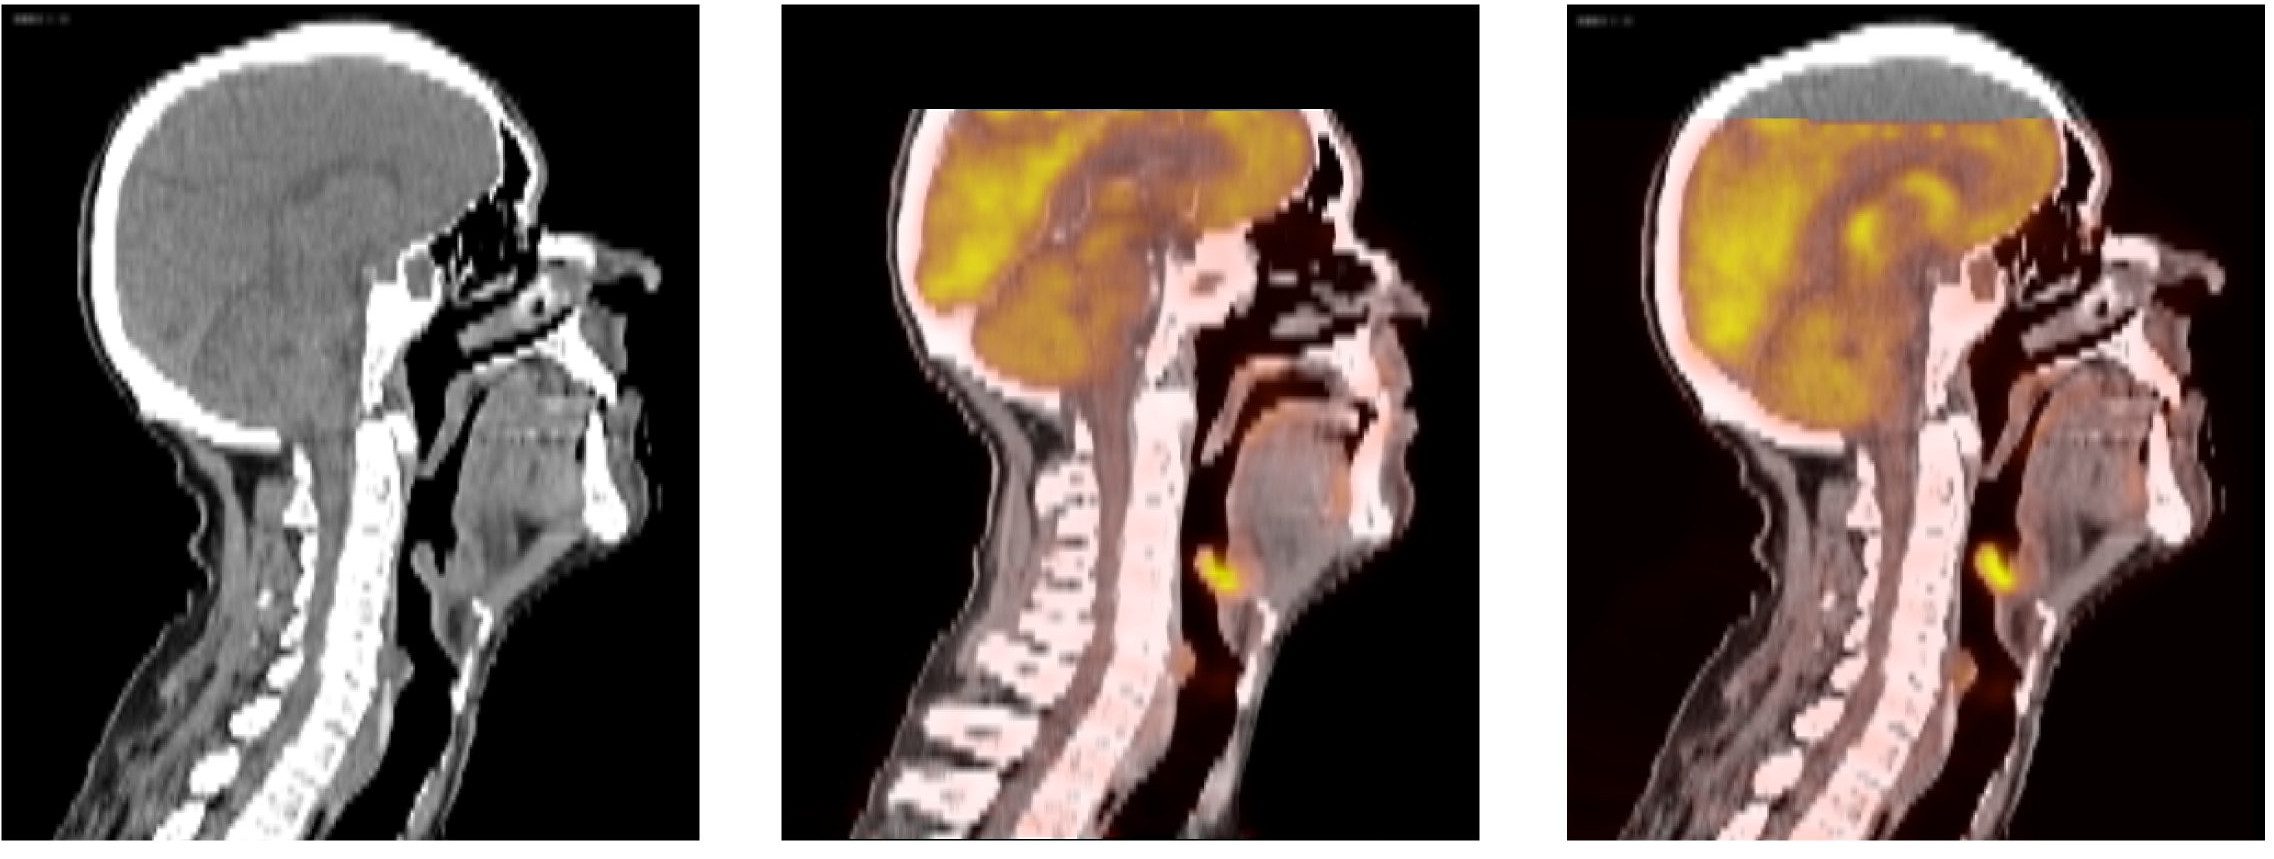
\includegraphics[width=1.0\textwidth]{figuras/fusion.png}
      \caption{Exemplo de fusão de imagens de diferentes modalidades. A primeira imagem é uma Tomografia Computadorizada,      
                a segunda é uma Tomografia por Emissão de Pósitrons (PET) e a terceira a fusão das duas.} 
      \source{https://www.leadtools.com/blog/medical-imaging/desktop-medical-viewer-control-updates/}{2}
    \end{center}
  \end{figure}
\end{frame}

\begin{frame}
  \begin{itemize}
    \item Os algoritmos de registro utilizam funções para mapear as imagens entre si 
    \item A natureza das funções nos permite classificá-los 
    \item A primeira classe utiliza funções simples como rotações e translações e os algoritmos pertencentes a ela
          realizam o registro rígido.
    \item Os algoritmos que alinham as imagens utilizando funções complexas, por exemplo aproximações por fluxo óptico
          ou funções radiais, são classificados como algoritmos de registro não-rígido.
  \end{itemize}
\end{frame}

\begin{frame}
  Os algoritmos de registro são altamente custosos computacionalmente por dois motivos:
  \begin{enumerate}
    \item A quantidade de etapas que são realizadas pré registro
    \item A quantidade de dados por estudos ou aplicação são muito grandes atualmente
  \end{enumerate}
  \begin{figure}
    \begin{center}
      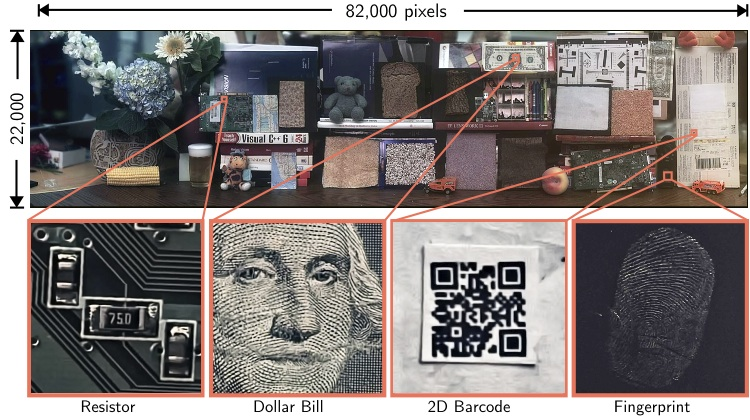
\includegraphics[width=0.6\textwidth]{figuras/teaser.jpg}
      \caption{Imagem \textit{Gigapixel}.} 
      \source{http://www.cs.columbia.edu/CAVE/projects/gigapixel/}{2}
    \end{center} 
  \end{figure}
\end{frame}

\begin{frame}
  A execução de um algoritmo de registro é composta de cinco passos:
  \begin{enumerate}
      \item Pré-processamento
      \item Detecção de características
      \item Correspondência de características
      \item Estimativa da função de transformação
      \item Reamostragem da Imagem Alvo
  \end{enumerate}
\end{frame}

\subsection{Motivação e Objetivos}

\begin{frame}
  Evolução da área de pesquisa:
  \begin{itemize}
      \item[2004] Primeiros trabalhos a unir registro não-rígido de imagens em \textit{Graphic Processing Units} (GPUs) 
                  \cite{strzodka2004image} \cite{kohn2006gpu}. Reportam aceleração de 4 e 12 vezes respectivamente
      \item[2007] As limitações da GPU são levadas em conta \cite{grossauer2008gpu}. Reporta a aceleração de 35 vezes
      \item[2009] Linguagens de programação para GPUs são utilizadas \cite{han2009gpu}. Reporta a aceleração de 15 vezes
      \item[2010] Algoritmos de registro desenvolvidos para GPU \cite{modat2010fast}. Reporta a execução do algoritmo em menos de 1 minuto
  \end{itemize}
\end{frame}

\begin{frame}
  O objetivo principal do trabalho é avaliar a portabilidade de algoritmos de registro não-rígido para execução em 
  GPUs.
  Os objetivos especificos do trabalho:
  \begin{itemize}
    \item Portar todas as etapas do registro para a arquitetura \textit{Single Instruction, Multiple Data} (SIMD) 
          \cite{patterson2013computer}, se assim elas ganharem eficiência
    \item Permitir o registro de múltiplas imagens simultaneamente
    \item Otimizar a ocupação dos recursos da GPU, preferencialmente entre as etapas do registro, com a finalidade de 
          minimizar a transferência de dados entre a CPU e a GPU
    \item Avaliar a eficiência comparado com a implementação em CPU
  \end{itemize}
\end{frame}

\section{Conceitos}
\subsection{Registro}

\begin{frame}
  \begin{itemize}
    \item O registro de imagens encontra um alinhamento geométrico (f) entre duas imagens, a Imagem Alvo (A) e a Imagem 
          Referência (R)
    \begin{align}\label{eq:defregistro}
      R(x,y) = A(f(x,y))
    \end{align}
    \item Ele percorre o espaço de parâmetros da função que representa o alinhamento em busca do melhor resultado
  \end{itemize}
\end{frame}

\begin{frame}
  \begin{figure}[H]
    \centering
    \begin{subfigure}[b]{0.49\textwidth}
      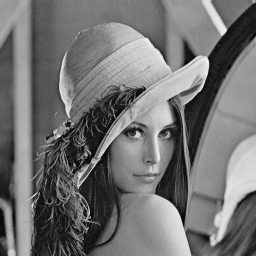
\includegraphics[width=1\textwidth]{figuras/static.png}
    \end{subfigure}
    \begin{subfigure}[b]{0.49\textwidth}
      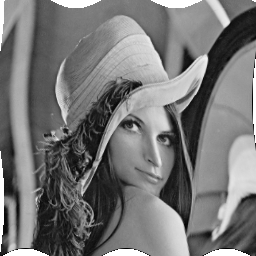
\includegraphics[width=1\textwidth]{figuras/lenaMoving.png}
    \end{subfigure}
    \caption{À esquerda a Imagem Referência. À direita a Imagem Alvo.}
  \end{figure}
\end{frame}

\begin{frame}
  1. Processamento:
  \begin{itemize}
    \item O pré-processamento é opcional e totalmente dependente da aplicação
    \item Filtros aplicados as imagens para diminuir a quantidade de ruido, ou realçar a imagem
    \item Detecção de bordas (e. g.\textit{Canny}\cite{canny1986computational} ou gradiente morfológico)
    \item Algoritmos de segmentação (e. g.\textit{Watersheds} \cite{vincent1991watersheds} ou limiarização)
  \end{itemize}
\end{frame}

\begin{frame}
  2. Detecção de características:
  \begin{itemize}
    \item Características são estruturas de destaque na cena ou objeto dentro das imagens
    \item Características devem ser facilmente identificadas
    \item São representadas na imagem por um conjunto de pixels
    \item Elas são divididas em três grupos:
    \begin{itemize}
      \item \textbf{Baseadas em Regiões}, regiões com diferenças de contraste marcante entre suas vizinhas
      \item \textbf{Baseadas em Retas}, interface entre duas regiões de uma imagem
      \item \textbf{Baseadas em Pontos}, representam a região na qual se encontram através de alguma propriedade
    \end{itemize}
  \end{itemize}
\end{frame}

\begin{frame}
  \begin{figure}[!h]
    \begin{center}
      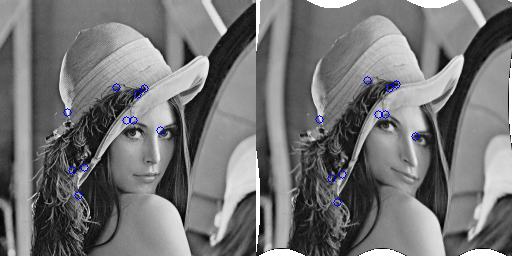
\includegraphics[width=1.0\textwidth]{figuras/Features.png}
      \caption{À esquerda as características da Imagem Referência. À direita as características da Imagem Alvo.}
    \end{center}
  \end{figure}
\end{frame}

\begin{frame}
  3. Correspondência de características:
  \begin{itemize}
    \item O próximo passo encontra correspondências entre as características das imagens Referência e Alvo
    \item Para cada grupo de correspondências existem métodos para a correspondência deles, com a adição de um outro:
    \begin{itemize}
      \item \textbf{Baseadas em Áreas}, utiliza janelas para mensurar áreas das duas imagens
      \item \textbf{Baseadas em Regiões}, compara o contorno das regiões
      \item \textbf{Baseadas em Retas}, pareia retas utilizando sua direção, comprimento e largura
      \item \textbf{Baseadas em Pontos}, utiliza descritores para encontrar as correspondências entre os pontos
    \end{itemize}
  \end{itemize}
\end{frame}

\begin{frame} 
  Dois algoritmos populares para detecção e correspondência de características:
  \begin{itemize}
    \item \textit{Scale Invariant Feature Transform} (SIFT) \cite{lowe2004distinctive}
    \item \textit{Speeded Up Robust Features} (SURF) \cite{bay2008speeded}
  \end{itemize}
  Os passos gerais executados por eles:
  \begin{itemize}
      \item Encontrar pontos \textbf{chave} no espaço de escala das imagens
      \item Determinar o vetor de descritores dos pontos \textbf{chave}
      \item Parear as características entre as imagens
    \end{itemize}
\end{frame}

\begin{frame}
  \begin{figure}[!h]
    \begin{center}
      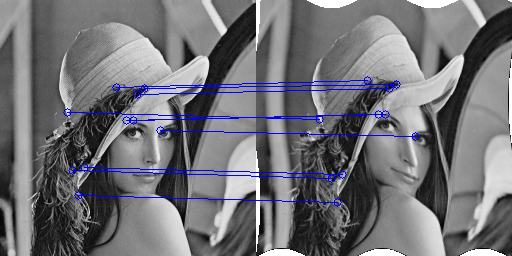
\includegraphics[width=1.0\textwidth]{figuras/MatchedFeatures.png}
      \caption{À esquerda as correspondências da Imagem Referência. À direita as correspondências da Imagem Alvo. 
               O SIFT foi o algoritmo utilizado.}
    \end{center}
  \end{figure}
\end{frame}

\begin{frame}
  4. Função de transformação:
  \begin{itemize}
    \item A primeira estimativa parte das correspondências 
    \item O algoritmo de registro passeia no espaço dos parâmetros em busca de um alinhamento ótimo
    \item O modelo de transformação deve ser escolhido conforme as necessidades da aplicação
      \begin{itemize}
        \item Fluxo óptico
        \item Informação Mútua
        \item Translações e rotações
      \end{itemize}
  \end{itemize}
\end{frame}

\begin{frame}
  5. Reamostragem da Imagem Alvo:
  \begin{itemize}
    \item A reamostragem da imagem Alvo aplica os parâmetros encontrados acima na transformação
    \item Reamostragem descrita pela equação abaixo
  \begin{align}\label{eq:reamostragem}
    F(x_i,y_j) = A(f(x_i,y_j))), \forall (i = 1, \dots, n_c), (j = 1, \dots, n_l)
  \end{align}
    \item Métodos de interpolação são necessários nesse passo
  \end{itemize}
\end{frame}

\begin{frame}
  \begin{figure}[H]
    \centering
    \begin{subfigure}[b]{0.49\textwidth}
      \includegraphics[width=1\textwidth]{figuras/rotateNN.png}
    \end{subfigure}
    \begin{subfigure}[b]{0.49\textwidth}
      \includegraphics[width=1\textwidth]{figuras/rotateBi.png}
    \end{subfigure}
    \caption{À esquerda imagem reamostrada usando o método de vizinho mais próximo. 
             À direita a imagem reamostrada usando o método bilinear.}
  \end{figure}
\end{frame}

\begin{frame}
  \begin{figure}[H]
    \centering
    \begin{subfigure}[b]{0.49\textwidth}
      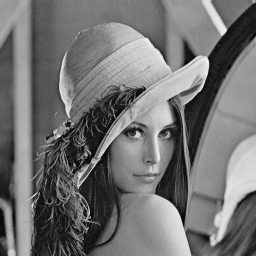
\includegraphics[width=1\textwidth]{figuras/static.png}
    \end{subfigure}
    \begin{subfigure}[b]{0.49\textwidth}
      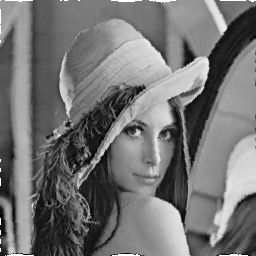
\includegraphics[width=1\textwidth]{figuras/lenaRegistrada.png}
    \end{subfigure}
    \caption{À esquerda a Imagem Referência. À direita a Imagem Registrada.}
  \end{figure}
\end{frame}

\subsection{GPGPU}

\begin{frame}
  \begin{itemize}
    \item \textit{High Performance Computing} (HPC) designa sistemas de alta capacidade de processamento e armazenamento
          de dados
    \item Uma instanciação de HPC pode ser feita com GPU
    \item Chamamos a aplicação de GPUs na solução de problemas computacionais de \textit{General-Purpose Computing on Graphics 
          Processing Units} (GPGPU)
  \end{itemize}
\end{frame}

\begin{frame}
  Sobre o processamento na GPU:
  \begin{itemize}
    \item Seguem a arquitetura de SIMD
    \item É composta de milhares de processadores, agrupados em \textit{Streaming Multiprocessors}
    \item As \textit{Threads} são organizadas em blocos, e eles são divididos para os SM
  \end{itemize}
\end{frame}

\begin{frame}[fragile]
  \begin{lstlisting}
    __global__ void VecAdd ( float* a, 
                             float* b, 
                             float* c) { 
      int i = threadIdx.x;
      a[i] = b[i] + c[i];        
    }
                              
    int main () {               
      ...                       
      VecAdd<<<1,M>>>(a, b, c);
      ...                       
    }                                 
  \end{lstlisting}
\end{frame}

\begin{frame}
  Limitações a se levar em conta:
  \begin{itemize}
    \item O acesso a blocos de memória é concorrente
    \item A transferência de dados entre GPU e CPU impacta no desempenho
    \item Evitar o número de bifurcações lógicas
  \end{itemize}
\end{frame}

\subsection{Algoritmos}

\begin{frame}
  \begin{itemize}
    \item Dois dos algoritmos mais representativos foram selecionados para serem avaliados
    \item \textit{Demons}
      \begin{itemize}
        \item Registra pequenas deformações com baixo custo computacional
        \item Modela a transformação ponto a ponto
      \end{itemize}
    \item TPS 
      \begin{itemize}
        \item Flexível
        \item Não utiliza as intensidades das imagens
      \end{itemize}
  \end{itemize}
\end{frame}

\begin{frame}
  Um dos algoritmos estudados de registro não-rígido estudado foi o \textit{Demons} \cite{thirion1995fast}
  \begin{itemize}
    \item O \textit{Demons} tem como base o modelo de atratores
    \item Ele adiciona o gradiente aos atratores para modelar a direção deles
  \end{itemize}
  \begin{figure}[H]
      \centering
      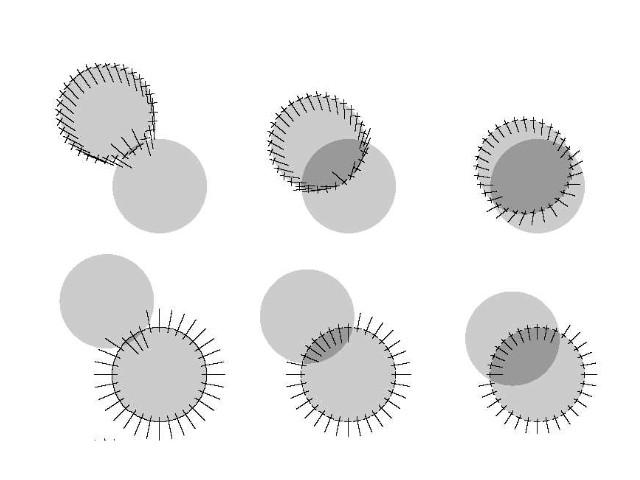
\includegraphics[width=0.45\textwidth]{figuras/demons.jpg}
      \caption{A primeira linha demonstra o sistema de atratores e a segunda o \textit{Demons}}
      \label{fig:demons}
  \end{figure}
\end{frame}

\begin{frame}
  O \textit{Demons} supõe que a transformação só movimenta os pixels, não muda suas intensidades e que as imagens 
  diferem de uma unidade de tempo. 
  \begin{align}
    \label{derivada}
    \vec{v} \cdot \vec{\nabla}R &= A - R, \ \text{onde} \ \vec{\nabla} R \ \text{é o gradiente de R} \\
    \vec{v} &= \frac{2(A - R)*(\vec{\nabla}R\vec{\nabla}A)}{(\vec{\nabla}R+\vec{\nabla}A)^2*(A - R)^2}
  \end{align}
\end{frame}

\begin{frame}
    O \textit{Demons} é um algoritmo iterativo. Como entrada ele recebe a imagem referência e alvo e possivelmente um campo
vetorial inicial. Cada iteração executa os passos:
\begin{enumerate}
    \item Para cada \textit{Demon} em $A_i$, calculamos $\vec{v_i}$, criando um novo campo vetorial $V_i$
    \item Aplicamos um filtro Gaussiano para retirar o ruído introduzido pelo processo em $V_i$
    \item Aplicamos $V_i$ em $A$ para obter $A_{i+1}$;
\end{enumerate}
\end{frame}

\begin{frame}
  O próximo algoritmo de registro não-rígido estudado foi o Thin Plate Splines (TPS) \cite{goshtasby2005}
  \begin{itemize}
    \item O TPS é uma função de interpolação radial
    \item As posições das características definem a função de interpolação
    \item A superfície é definida pela seguinte equação\cite{bookstein1989principal}:
  \end{itemize}
  \begin{align}
  \begin{split}
      f(x,y) &= A_0 + A_1x + A_2y + \sum_{i=0}^n F_i r_i^2 ln r_i^2 \\
      r_i^2 &= (x-x_i)^2 + (y-y_i)^2 + d^2
  \end{split}    
  \end{align}
\end{frame}

\begin{frame}
  O TPS determina os valores das variáveis $A_0, A_1, A_2$ e dos $F_i$:
  \begin{align}
  \begin{split}
      \sum_{i=1}^n F_i &= 0, \sum_{i=1}^n F_ix = 0, \sum_{i=1}^n F_iy = 0 \\
      f(x_1,y_1) &= A_0 + A_1x + A_2y + \sum_{i=0}^n F_i r_{i1}^2 ln r_{i1}^2 \\
      \vdots \\
      f(x_n,y_n) &= A_0 + A_1x + A_2y + \sum_{i=0}^n F_i r_{in}^2 ln r_{in}^2
  \end{split}
  \end{align}
\end{frame}

\section{Experimentos}
\subsection{Experimentos}

\begin{frame}
   \begin{columns}[c]
      \column{.5\textwidth}
      Para os experimentos uma das imagens padrão do software BioImage \cite{papademetris2005bioimage} foi utilizada.
      As deformações aplicadas a imagem de teste foram baseadas no trabalho Zargorchev \cite{zagorchev2006comparative}.
      \column{.5\textwidth}
        As transformações serão aplicadas à grade abaixo.
        \begin{figure}[!h]
          \begin{center}
            
\includegraphics[width=0.8\textwidth]{figuras/grid.png}
            \caption{Grade sem deformações.}
          \end{center}
        \end{figure}
    \end{columns}
\end{frame}

\begin{frame}
   \begin{columns}[c]
      \column{.5\textwidth}
        A primeira transformação é dada por:
        \begin{align}
        \begin{split}
            X &= x - 8sen(x/32) \\
            Y &= y + 4cos(x/16)
        \end{split} 
        \end{align}
      \column{.5\textwidth}
        \begin{figure}[!h]
          \begin{center}
            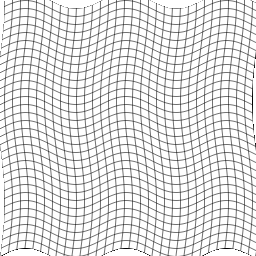
\includegraphics[width=0.8\textwidth]{figuras/gridSin.png}
            \caption{Grade deformada pela função senoidal.}
          \end{center}
        \end{figure}
    \end{columns}
\end{frame}

\begin{frame}
   \begin{columns}[c]
      \column{.5\textwidth}
        A próxima transformação é dada por:
        \begin{align}
        \begin{split}
            X &= x + 50(x-n_c)/r \\
            Y &= y + 50(y-n_l)/r 
        \end{split} 
        \end{align}
      \column{.5\textwidth}
        \begin{figure}[!h]
          \begin{center}
            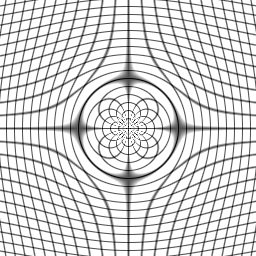
\includegraphics[width=0.8\textwidth]{figuras/gridDist.png}
            \caption{Grade deformada pela função de distância inversa.}
          \end{center}
        \end{figure}
    \end{columns}
\end{frame}

\begin{frame}
   \begin{columns}[c]
      \column{.5\textwidth}
        A última transformação é dada pela combinação das duas:
        \begin{align}
        \begin{split}
            X &= x-8sen(x/32)+50(x-n_c)/r \\
            Y &= y+4cos(x/16)+50(y-n_l)/r
        \end{split} 
        \end{align}
      \column{.5\textwidth}
        \begin{figure}[!h]
          \begin{center}
            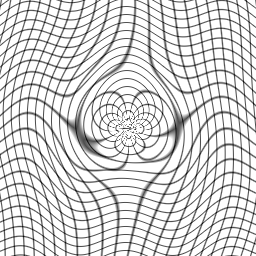
\includegraphics[width=0.8\textwidth]{figuras/movingImageDistSin.png}
            \caption{Grade deformada pela combinação das duas anteriores.}
          \end{center}
        \end{figure}
    \end{columns}
\end{frame}

\subsection{Resultados}

\begin{frame}
  \begin{picture}(320,250)
    \put(40,155){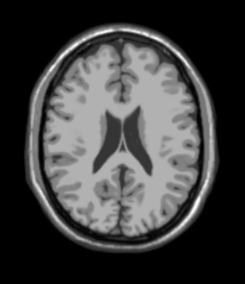
\includegraphics[scale=0.35]{figuras/screen.png}}
    \put(40,145){\begin{minipage}[t]{0.35\linewidth}{Imagem Referência}\end{minipage}}
    \put(150,155){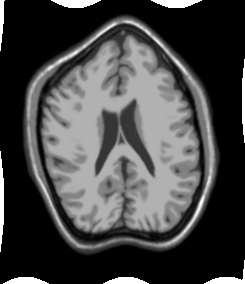
\includegraphics[scale=0.35]{figuras/movingImageSin.png}}
    \put(150,145){\begin{minipage}[t]{0.35\linewidth}{Senoidal}\end{minipage}}
    \put(40,40){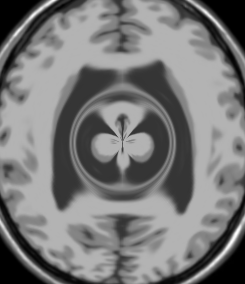
\includegraphics[scale=0.35]{figuras/movingImageDist.png}}
    \put(40,30){\begin{minipage}[t]{0.35\linewidth}{Distância inversa}\end{minipage}}
    \put(150,40){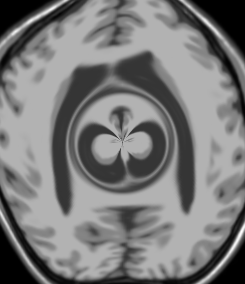
\includegraphics[scale=0.35]{figuras/movingImageSinDist.png}}
    \put(150,30){\begin{minipage}[t]{0.35\linewidth}{Combinação}\end{minipage}}
  \end{picture}
\end{frame}

\begin{frame}
  \begin{figure}[H]
    \centering
    \begin{subfigure}[b]{0.49\textwidth}
      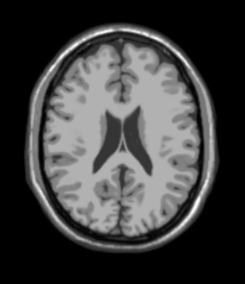
\includegraphics[width=1\textwidth]{figuras/screen.png}
    \end{subfigure}
    \begin{subfigure}[b]{0.49\textwidth}
      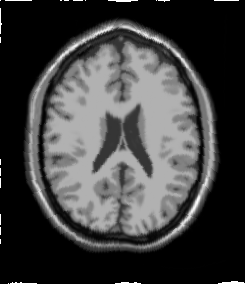
\includegraphics[width=1\textwidth]{figuras/resultSin.png}
    \end{subfigure}
    \caption{À esquerda a Imagem Referência. À direita a imagem registrada pelo TPS.}
  \end{figure}
\end{frame}

\begin{frame}
  \begin{figure}[H]
    \centering
    \begin{subfigure}[b]{0.49\textwidth}
      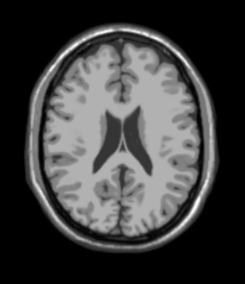
\includegraphics[width=1\textwidth]{figuras/screen.png}
    \end{subfigure}
    \begin{subfigure}[b]{0.49\textwidth}
      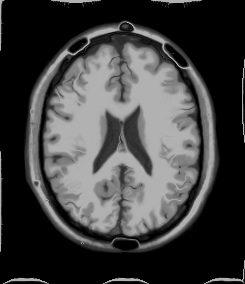
\includegraphics[width=1\textwidth]{figuras/resultSinDemon.png}
    \end{subfigure}
    \caption{À esquerda a Imagem Referência. À direita a imagem registrada pelo \textit{Demons}.}
  \end{figure}
\end{frame}

\begin{frame}
  \begin{figure}[H]
    \centering
    \begin{subfigure}[b]{0.49\textwidth}
      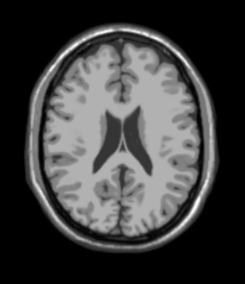
\includegraphics[width=1\textwidth]{figuras/screen.png}
    \end{subfigure}
    \begin{subfigure}[b]{0.49\textwidth}
      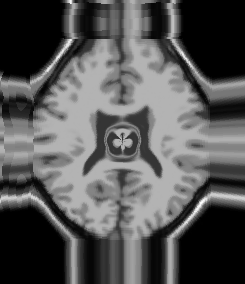
\includegraphics[width=1\textwidth]{figuras/resultDist.png}
    \end{subfigure}
    \caption{À esquerda a Imagem Referência. À direita a imagem registrada pelo TPS.}
  \end{figure}
\end{frame}

\begin{frame}
  \begin{figure}[H]
    \centering
    \begin{subfigure}[b]{0.49\textwidth}
      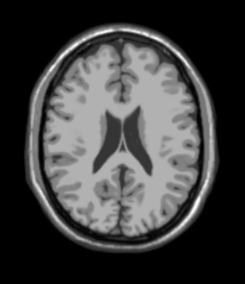
\includegraphics[width=1\textwidth]{figuras/screen.png}
    \end{subfigure}
    \begin{subfigure}[b]{0.49\textwidth}
      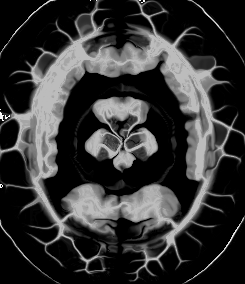
\includegraphics[width=1\textwidth]{figuras/resultDistDemons.png}
    \end{subfigure}
    \caption{À esquerda a Imagem Referência. À direita a imagem registrada pelo \textit{Demons}.}
  \end{figure}
\end{frame}

\begin{frame}
  \begin{figure}[H]
    \centering
    \begin{subfigure}[b]{0.49\textwidth}
      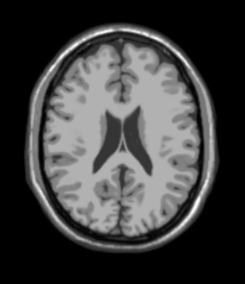
\includegraphics[width=1\textwidth]{figuras/screen.png}
    \end{subfigure}
    \begin{subfigure}[b]{0.49\textwidth}
      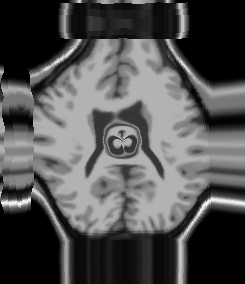
\includegraphics[width=1\textwidth]{figuras/resultDistSin.png}
    \end{subfigure}
    \caption{À esquerda a Imagem Referência. À direita a imagem registrada pelo TPS.}
  \end{figure}
\end{frame}

\begin{frame}
  \begin{figure}[H]
    \centering
    \begin{subfigure}[b]{0.49\textwidth}
      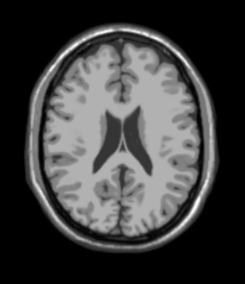
\includegraphics[width=1\textwidth]{figuras/screen.png}
    \end{subfigure}
    \begin{subfigure}[b]{0.49\textwidth}
      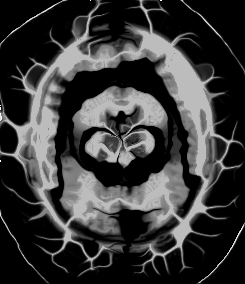
\includegraphics[width=1\textwidth]{figuras/resultSinDistDemon.png}
    \end{subfigure}
    \caption{À esquerda a Imagem Referência. À direita a imagem registrada pelo \textit{Demons}.}
  \end{figure}
\end{frame}

\begin{frame}
  \begin{table}[H]
    \begin{center}
      \begin{tabular}{|l|c|c|c|c|}
        \hline
        Algoritmo & Tempo médio & desvio padrão & máximo & mínimo \\
        \hline
        \textit{Demons} & 686,42 s & 27,71 s & 740,21 s & 632,90 s \\
        \hline
        TPS & 329,19 s & 44,57 s & 432,75 s & 289,43 s \\
        \hline
      \end{tabular}
      \caption{Tempo de execução dos testes com a deformação senoidal}
      \label{table:tps}
    \end{center}
  \end{table}
  \begin{table}[H]
    \begin{center}
      \begin{tabular}{|l|c|}
        \hline
        Algoritmo & Tempo Assintótico de execução \\
        \hline
        \textit{Demons} &$\mathcal{O}(x*n_l^2*n_c^2)$ \\
        \hline
        TPS             &$\mathcal{O}(\frac{4}{3}n_{cp}^3+n_l*n_c*n_{cp})$\\
        \hline
      \end{tabular}
      \caption{Tempo Assintótico de execução dos algoritmos}
      \label{table:tps}
    \end{center}
  \end{table}
\end{frame}

\section{Proposta}
\subsection{Proposta}

\begin{frame}
  Os próximos passos para completar o estudo são, em prioridade:
  \begin{enumerate}
    \item Avaliar a portabilidade do SIFT e SURF para GPU
    \item Criar uma versão GPGPU dos algoritmos utilizando a linguagem CUDA
    \item Possibilitar a execução com múltiplas entradas (imagens)
    \item Escrever um artigo científico
    \item Escrever a dissertação
  \end{enumerate}
  \begin{table}
  \begin{center}
  \begin{small}
  \begin{tabular}{|c|c|c|c|c|c|c|c|} 
  \hline
  \emph{Tarefa} &
  Março & 
  Abril & 
  Maio &  
  Junho & 
  Julho &
  Agosto & 
  Setembro \\ \hline
  \textbf{1} & X &  &  &  &  &  &  \\ \hline 
  \textbf{2} & X & X & X &  &  &  &  \\ \hline 
  \textbf{3} &  &  & X & X &  &  &  \\ \hline 
  \textbf{4} & X & X & X &  &  &  &  \\ \hline 
  \textbf{5} &  &  & X & X & X & X & X \\ \hline 
  \end{tabular}
  \caption{Cronograma.}
  \label{tab:tab:F5}
  \end{small}
  \end{center}
  \end{table}
\end{frame}

\section{Bibliografia}
\subsection{}

\begin{frame}[allowframebreaks]
  \frametitle{Referências}    
  \framesubtitle{}
  \bibliographystyle{alpha-ime}
  \bibliography{bibliografia}{}
\end{frame}
\end{document}